\documentclass[10pt,a4paper]{report}
%\usepackage[utf8]{inputenc}
\usepackage[latin1]{inputenc}
\usepackage{amsmath}
\usepackage{amsfonts}
\usepackage{amssymb}
\usepackage{multicol, blindtext}
\usepackage{textcomp}
\usepackage{graphicx}
\usepackage{lipsum}

\title{Exemplos de Aplica��es em Comunica��o Digital usando $MatLab^{\copyright}$}

\begin{document}



%\title{Medi��o de Velocidade usando um Sensor de Luminosidade}

\author{Danilo Souza - 10080000801, Hugo Santos - 10080000701, Welton Ara�jo - 10080000501}
%Matr�culas: {10080000801, 10080000701, 10080000501}
%\thanks{Engenharia da Computa\c{c}\~ao, Universidade Federal do Par\'a, Bel\'em-PA, Brasil}
\maketitle

\tableofcontents


%Emails: \{dhcsouza, huggosan, weltonmaxx007\}@gmail.com\\


\chapter{C�lculo dos Coeficientes da S�rie de Fourier}

\section{Funcionamento do Script}
	O script � utilizado para fazer o c�lculo num�rico dos coeficientes da s�rie de Fourier da fun��o $\Delta(t/2)$, utilizando a f�rmula da transformada inversa mostrada na equa��o \ref{eq:formcoef} . O algoritmo do programa est� definido abaixo.

	\[ t_{p} = \dfrac{\pi}{w_{d}} \]
	
	\[ \dfrac{C(s)}{R(s)} = \dfrac{kw_{n}^{2}}{s^{2} + 2\xi w_{n} s + w^{2}_{n}} \]

	\[ \dfrac{C(s)}{R(s)} = \dfrac{K}{s^{2} + (1+KK_{h})s + K} \]

	\[ w_{d} = w_{n}\sqrt[]{1-\xi^{2}} \]
	
	Os efeitos do $\xi$ foram relacionados ao tempo de estabiliza��o e � tens�o de pico. O comportamento � mostrado nas Figuras \ref{fig:i_w2_k8_e1}, \ref{fig:i_w2_k8_e07} e \ref{fig:i_w2_k8_e02} para, respectivamente, os valores $\xi$ = 1, 0.7, 0.2 e $w_{n}$ = 2.
	

\begin{figure}[h]
\centering
	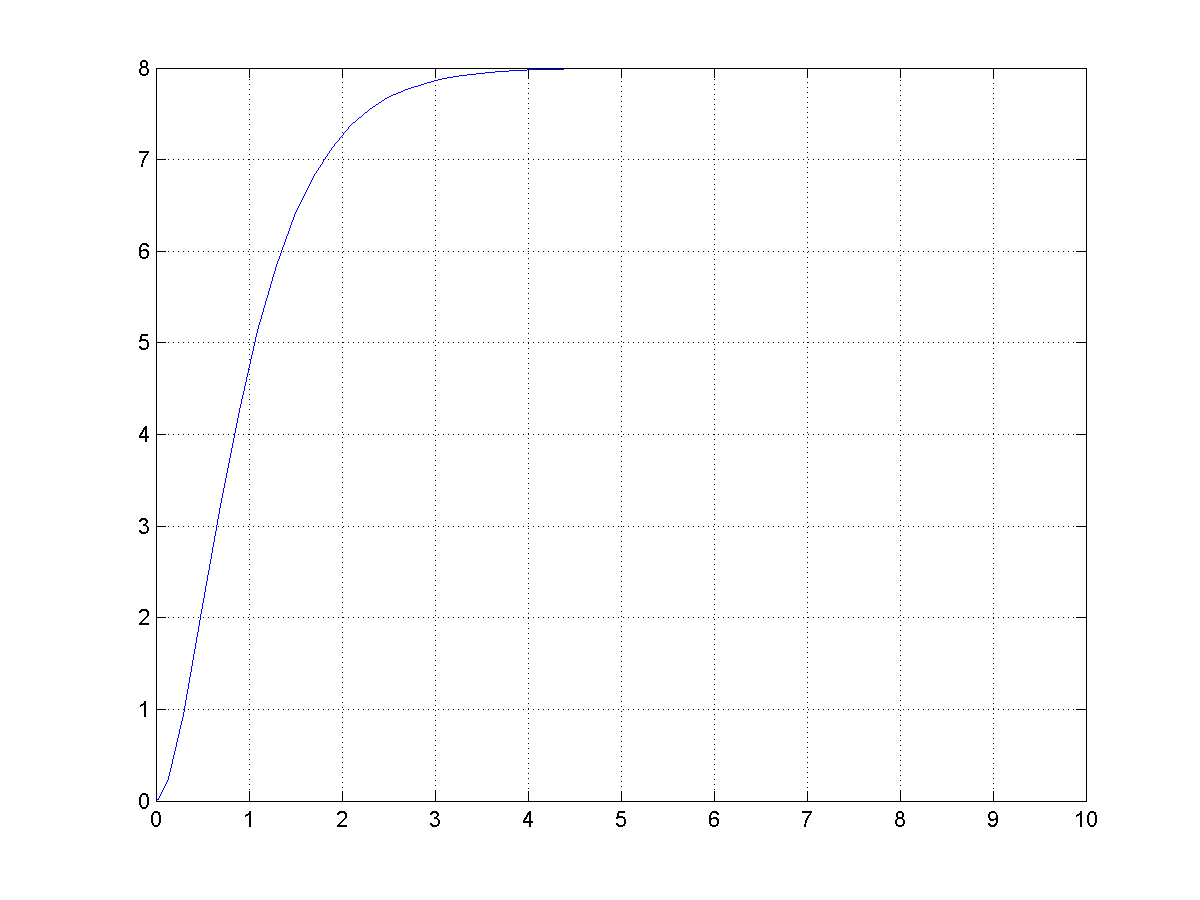
\includegraphics[scale=0.5]{./pictures/i_w2_k8_e1.png}
	\caption{Para $w_{n}$=2, k = 8 e $\xi$ = 1}
	\label{fig:i_w2_k8_e1}
\end{figure}
\begin{figure}[h]
\centering
	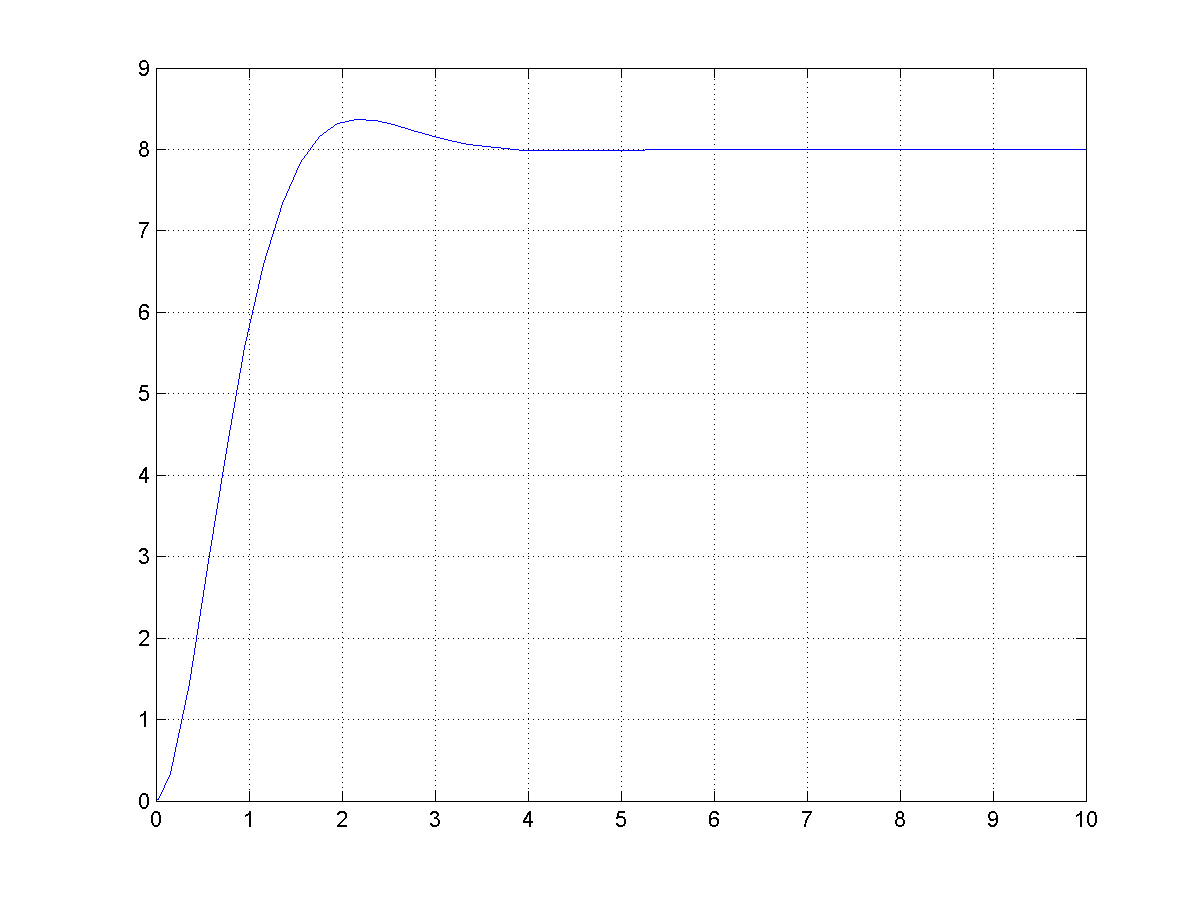
\includegraphics[scale=0.5]{./pictures/i_w2_k8_e07.png}
	\caption{Para $w_{n}$=2, k = 8 e $\xi$ = 0.7}
	\label{fig:i_w2_k8_e07}
\end{figure}
\begin{figure}[h]
\centering
	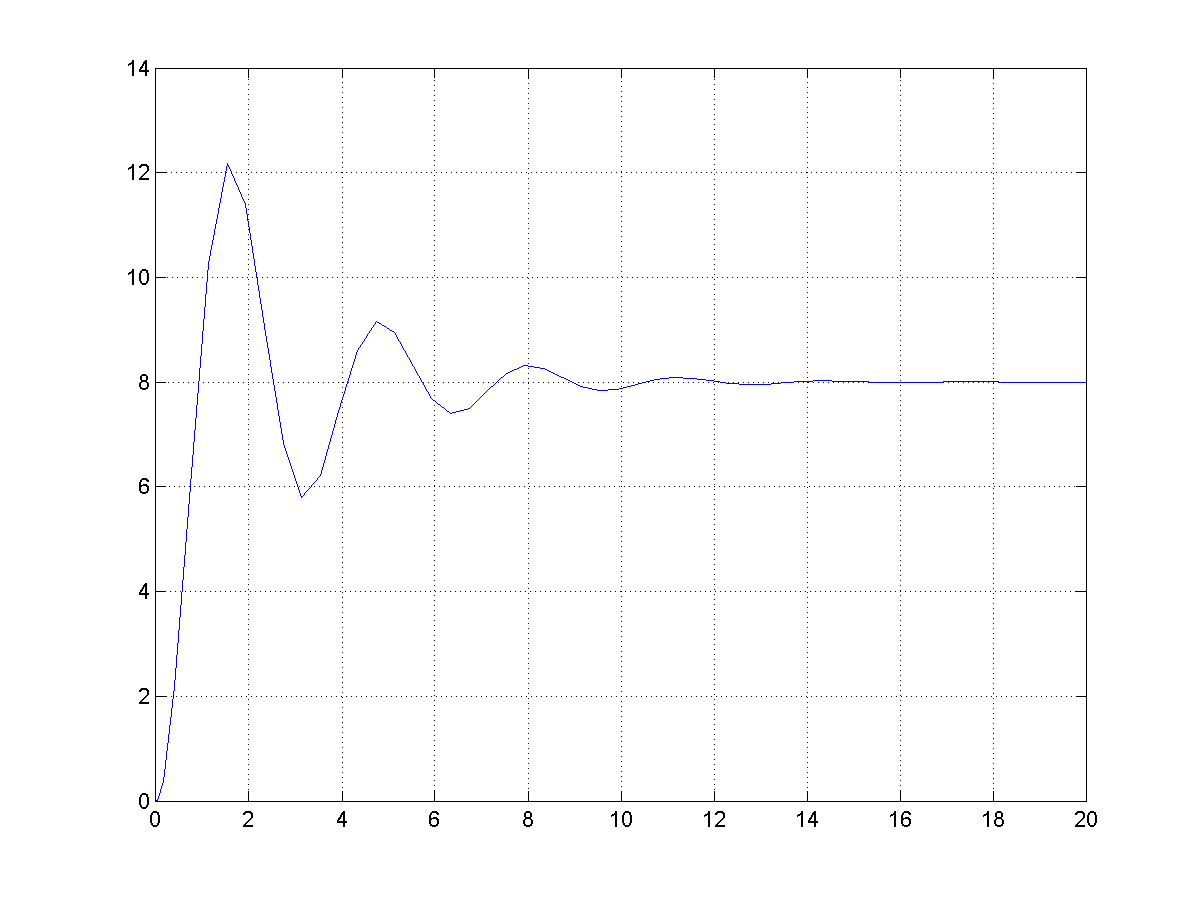
\includegraphics[scale=0.5]{./pictures/i_w2_k8_e02.png}
	\caption{Para $w_{n}$=2, k = 8 e $\xi$ = 0.2}
	\label{fig:i_w2_k8_e02}
\end{figure}

	Os efeitos do $w_{n}$ tiveram grande influ�ncia sobre o tempo de resposta, pois com um valor maior, o $T_{p}$ diminue. As Figuras \ref{fig:i_w10_k8_e1}, \ref{fig:i_w10_k8_e07} e \ref{fig:i_w10_k8_e02} mostram o comportamento do sinal para, respectivamente, os valores $\xi$ = 1, 0.7, 0.2 e $w_{n}$ = 10.

\begin{figure}[h]
\centering
	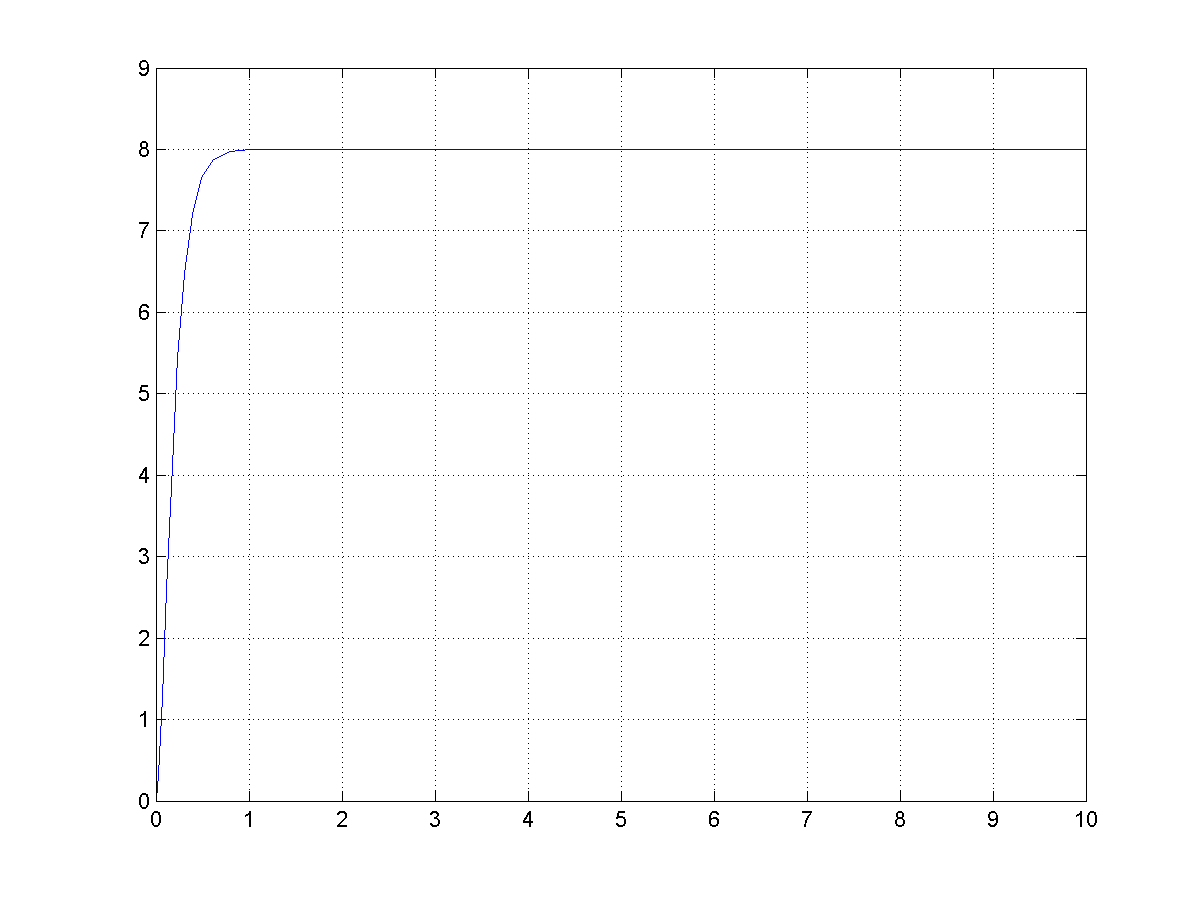
\includegraphics[scale=0.75]{./pictures/ii_w10_k8_e1.png}
	\caption{Para $w_{n}$=10, k = 8 e $\xi$ = 1}
	\label{fig:i_w10_k8_e1}
\end{figure}
\begin{figure}[h]
\centering
	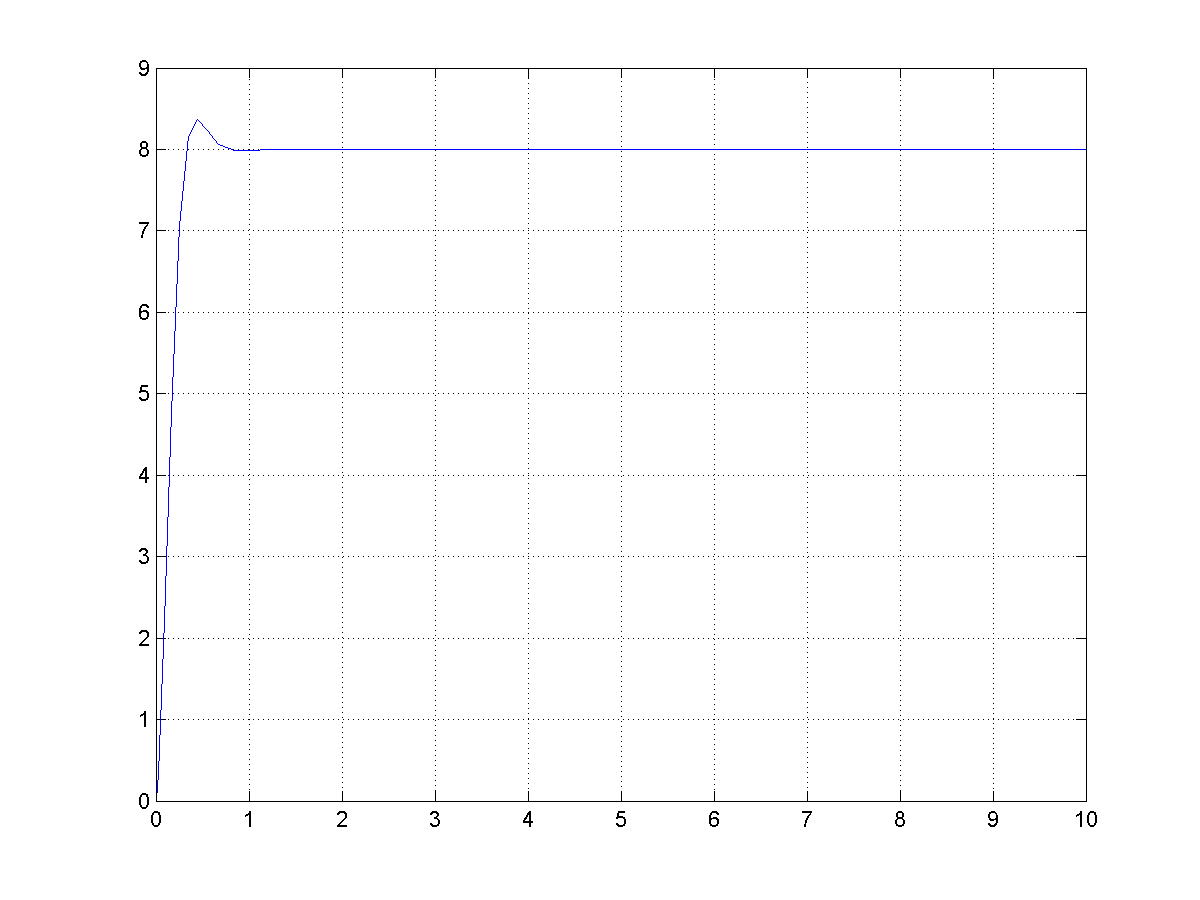
\includegraphics[scale=0.75]{./pictures/ii_w10_k8_e07.png}
	\caption{Para $w_{n}$=10, k = 8 e $\xi$ = 0.7}
	\label{fig:i_w10_k8_e07}
\end{figure}
\begin{figure}[h]
\centering
	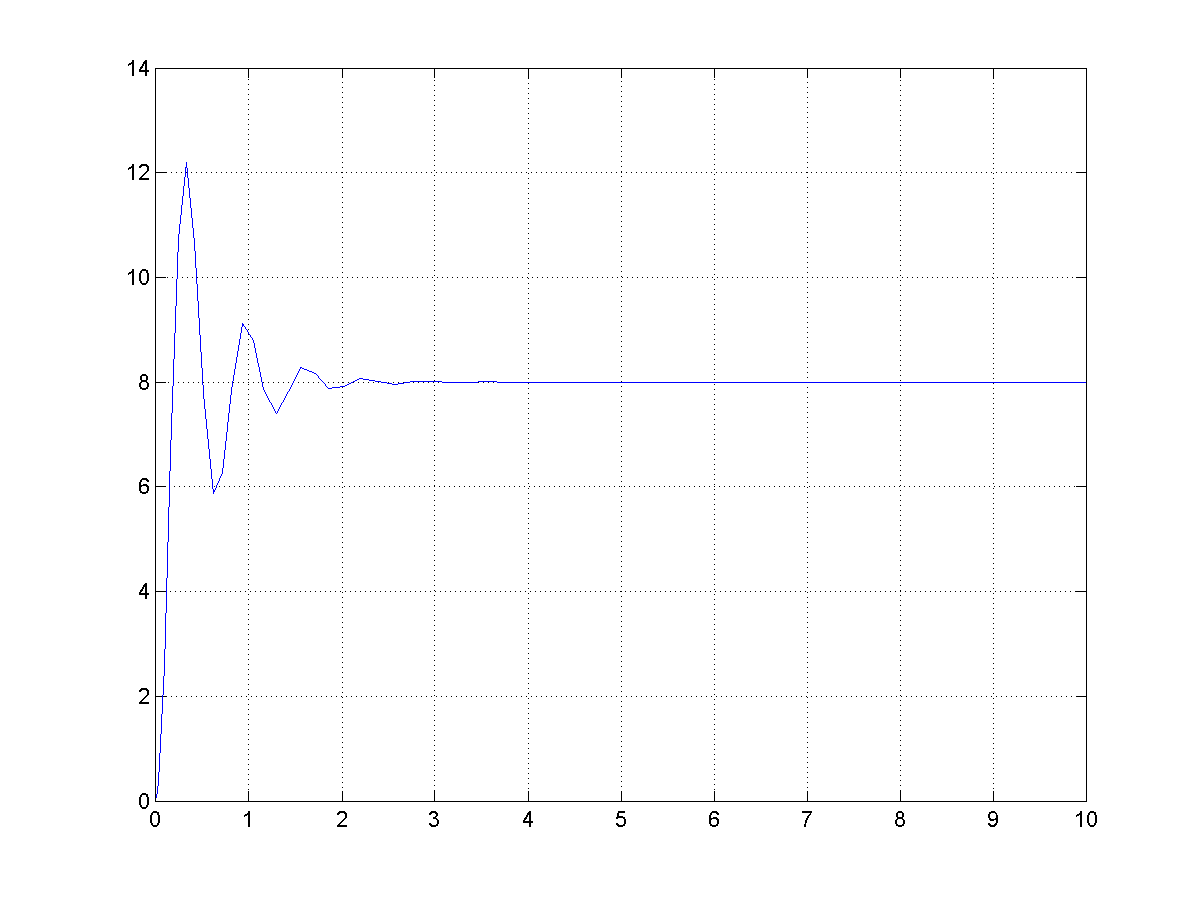
\includegraphics[scale=0.75]{./pictures/ii_w10_k8_e02.png}
	\caption{Para $w_{n}$=10, k = 8 e $\xi$ = 0.2}
	\label{fig:i_w10_k8_e02}
\end{figure}

\section{Resultados}
Se os valores de $T_{0}$ e $T_{s}$ forem modificados, o sinal perde a caracter�stica que realmente 


\end{document}